\newthought{\textbf{Jihan Dwi Sarah - 2020903430015 - TRKJ 3B}}


\newday{\textbf{1 - 2 Desember 2022} - Instalasi Hadoop}
\begin{enumerate}
\item Kendala dan Solusi
% jelaskan kendala dan penyebab yang dialami saat mengikuti praktikum serta solusi atau langkah-langkah yang telah dilakukan
\newline Pada pertemuan hari ini, kegiatan yang dilakukan adalah menginstall Apache Hadoop. Selama praktikum tidak mengalami kendala.

\item Kesimpulan \\
% berikan kesimpulan dari praktikum yang telah dikerjkan
Berhasil melakukan instalasi java tanpa ada bug atau error serta instalasi hadoop berikut ini gambar hasil verifikasi instalasi java version dan hadoop version 

\begin{figure}[!ht]
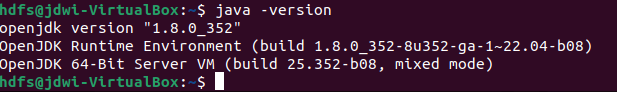
\includegraphics[width=\textwidth]{JihanDwiSarah/Java-version(Jihan)}
\caption{Verifikasi Hasil Instalasi Java}
\label{gam:Java-version(Jihan)}
\end{figure} 

\begin{figure}[!ht]
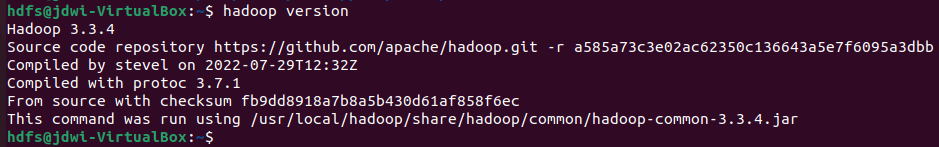
\includegraphics[width=\textwidth]{JihanDwiSarah/Hadoop-version(Jihan)}
\caption{Verifikasi Hasil Instalasi Hadoop}
\label{gam:Hadoop-version(Jihan)}
\end{figure}
\end{enumerate}


\newday{\textbf{8 - 9 Desember 2022} - Konfigurasi Hadoop}
\begin{enumerate}
\item Kendala dan Solusi \\
% jelaskan kendala dan penyebab yang dialami saat mengikuti praktikum serta solusi atau langkah-langkah yang telah dilakukan
Pada pertemuan hari ini, kegiatan yang dilakukan adalah mengkonfigurasi Apache Hadoop. Selama praktikum tidak mengalami kendala.

\item Kesimpulan \\
% berikan kesimpulan dari praktikum yang telah dikerjkan
Berhasil mengkonfigurasi beberapa file Hadoop sehingga memudahkan dalam memonitoring ekosistem Hadoop yang telah diinstall. Berikut ini gambar bukti keberhasilan praktikum. 

\begin{figure}[!ht]
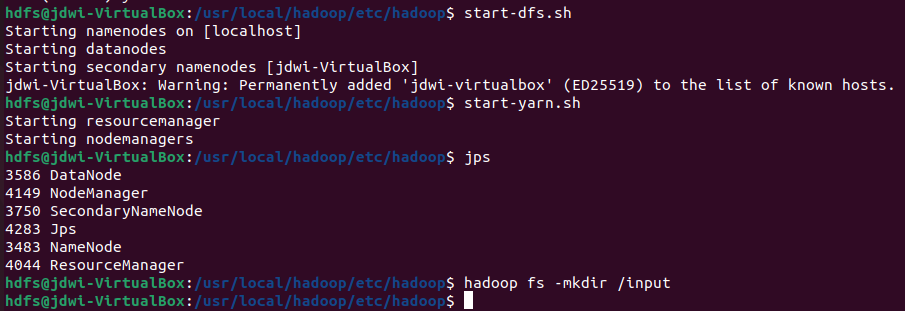
\includegraphics[width=\textwidth]{JihanDwiSarah/perintah-jps(jihan)}
\caption{Hasil perintah jps}
\label{gam:perintah-jps(jihan)}
\end{figure} 


\begin{figure}[!ht]
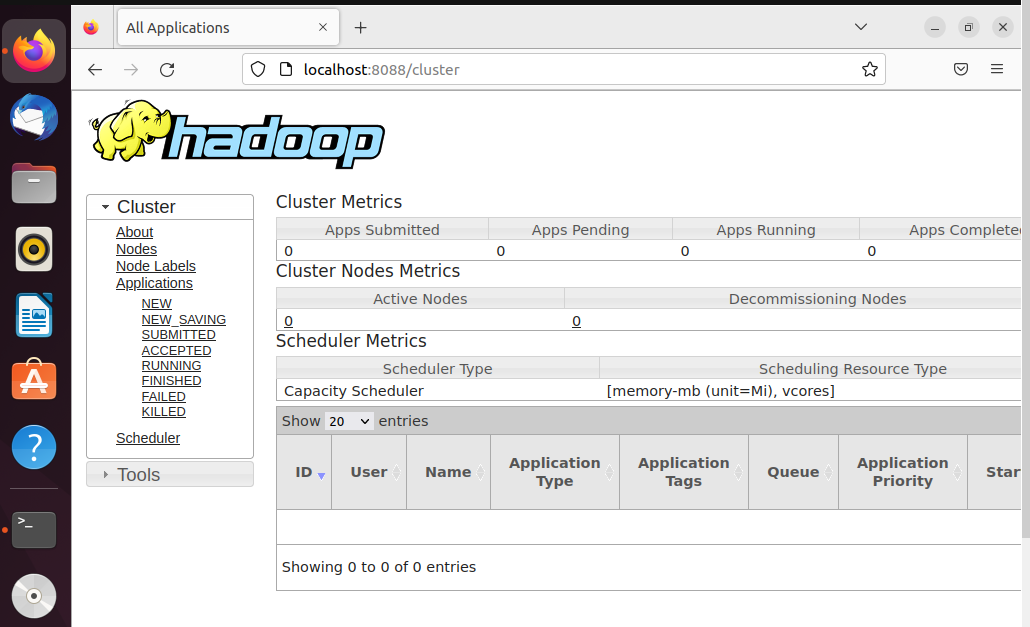
\includegraphics[width=\textwidth]{JihanDwiSarah/Akses-web-browser-8088(Jihan)}
\caption{Akses melalui web browser dengan alamat http://localhost:8088}
\label{gam:Akses-web-browser-8088(Jihan)}
\end{figure} 

\begin{figure}[!ht]
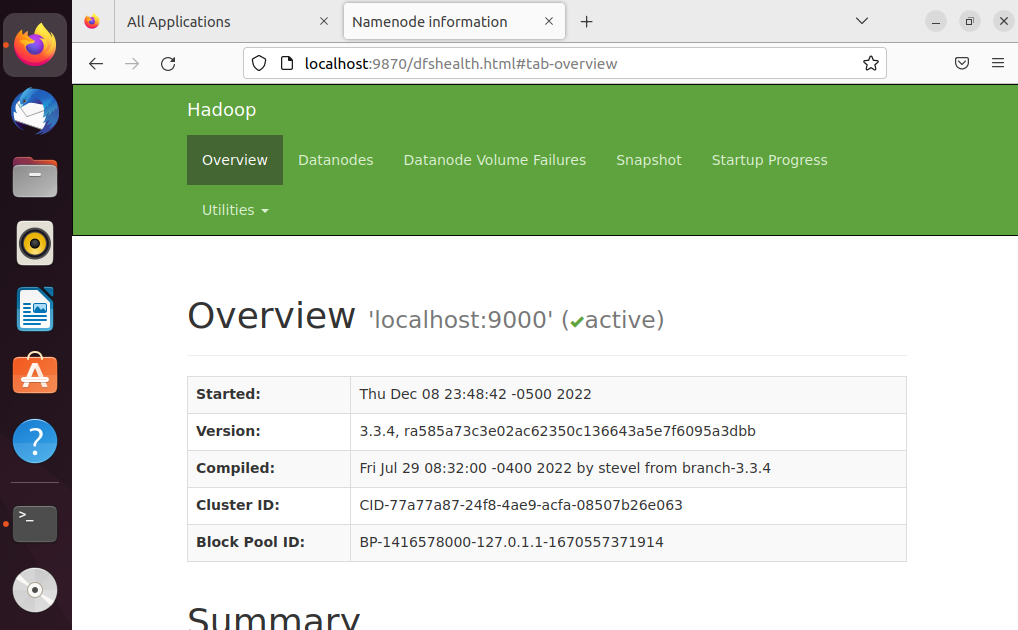
\includegraphics[width=\textwidth]{JihanDwiSarah/Akses-web-browser-9870(Jihan)}
\caption{Akses melalui web browser dengan alamat http://localhost:9870}
\label{gam:Akses-web-browser-9870(Jihan)}
\end{figure} 
\end{enumerate}

\newday{\textbf{15 Desember 2022} - WordCount Bawaan Hadoop}
\begin{enumerate}
\item Kendala dan Solusi \\
% jelaskan kendala dan penyebab yang dialami saat mengikuti praktikum serta solusi atau langkah-langkah yang telah dilakukan
Pada pertemuan hari ini, kegiatan yang dilakukan adalah mencoba program bawaan Hadoop untuk memahami bagaimana
proses dan cara kerja Hadoop dalam memproses data input hingga menghasilkan sebuah output. Selama praktikum tidak mengalami kendala.

\item Kesimpulan\\
% berikan kesimpulan dari praktikum yang telah dikerjkan
Berhasil mencoba program bawaan Hadoop yaitu program menghitung jumlah kata dalam data input yang diberikan.Berikut ini gambar bukti keberhasilan praktikum. 
\begin{figure}[!ht]
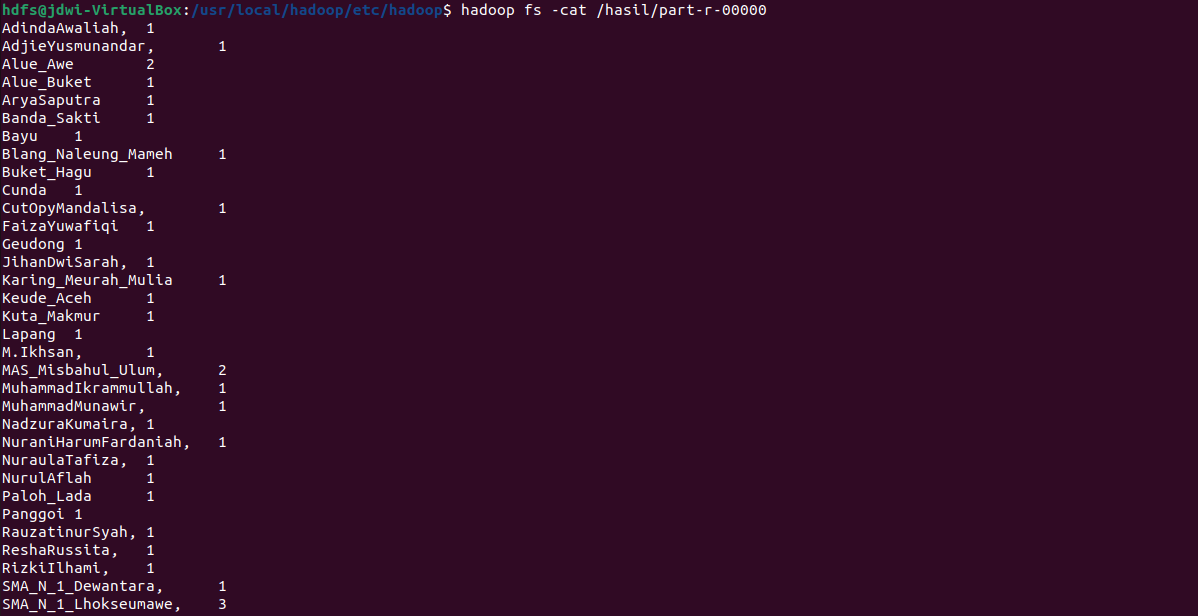
\includegraphics[width=\textwidth]{JihanDwiSarah/WordCount bawaan-Hadoop(jihan)}
\caption{Akses melalui web browser dengan alamat http://localhost:9870}
\label{gam:WordCount bawaan-Hadoop(jihan)}
\end{figure}
\end{enumerate}

\newday{\textbf{} - }
\begin{enumerate}
\item Kendala dan Solusi \\
% jelaskan kendala dan penyebab yang dialami saat mengikuti praktikum serta solusi atau langkah-langkah yang telah dilakukan


\item Kesimpulan\\
% berikan kesimpulan dari praktikum yang telah dikerjkan

\end{enumerate}

